%!TEX program = lualatex
\documentclass[14pt]{constructor-thesis}

\usepackage[backend=bibtex]{biblatex}
\usepackage{tikz}
\usepackage{import}
\addbibresource{thesis.bib}

\begin{document}
% Год, город, название университета и факультета предопределены,
% но можно и поменять.
% Если англоязычная титульная страница не нужна, то ее можно просто удалить.
\filltitle{en}{
  chair              = {Bachelor of Science \\ Computer Science},
  title              = {Mechanizing semantics of graph query languages in Coq},
  author             = {Semen Panenkov},
  supervisorPosition = {Prof.},
  supervisor         = {Anton Podkopaev},
  reviewerPosition   = {},
  reviewer           = {},
  chairHeadPosition  = {Dr.},
  chairHead          = {Stanislav Protasov},
}
\maketitle
\tableofcontents
% У введения нет номера главы
\section*{Introduction}

Databases have come a long way since their inception, and today we have a plethora of database types available, each designed to serve a particular use-case~\cite{database-types}. One of the more recent types to gain popularity are graph databases.

As the name suggests, graph databases represent data using graphs. While the idea of representing data with graphs isn't new with solutions developed as early as the mid-1960s, the first enterprise-ready ACID-compliant transactional database only emerged in 2007 with the release of Neo4j~\cite{enwiki:1146498781}. Since then, many graph databases such as Amazone Neptune, RedisGraph and NebulaGraph have sprung up~\cite{enwiki:1146498781}, with successful applications in various fields including recommendation services, fraud detection in finance~\cite{neo4j:use-cases} and even investigations of corruption schemes~\cite{icij:offshoreleaks}.

However, despite the growing popularity of graph databases, the lack of a standardized query language poses significant challenges to their wider adoption. The graph database community has developed Graph Query Language (GQL) to address this need. Nevertheless, standardizing GQL is challenging due to its complexity and constant expansion, and can result in errors and ambiguities even after thorough reviews~\cite{cpp-std-verified}. Furthermore, given the declarative nature of GQL, the database needs to determine how to fetch the data described in the query, leading to a greater number of possible implementations. This even poses into question the very existence of a realistic implementation.

% In fact, graph databases translate a query into an intermediate representation called \textbf{execution plan}, which is just a sequence of operations that need to be performed in order to evaluate the query. These operations inspect the graph and produce intermediate results that are later transformed by subsequent operations. This solution draws inspiration from relational databases world, where such approach has proven to be successful.

% However, this still leaves a lot of space to the implementators of the standard. For example, Neo4j and RedisGraph use different sets of operations and implement them differently. The former divides a query into a large sequence of small and simple operations while the latter covers with one complex operation the bigger part of a query but its operations are heavily optimized using linear algebra. The situation is further complicated by the fact that the translation process itself is complex and contains a lot of subtle details.

To address these challenges, we propose a formal approach to standardizing GQL and ensuring the correctness of the key details of query evaluation. Specifically, we aim to demonstrate the correctness of the way that Neo4j and RedisGraph, our reference databases, translate queries to execution plans. To achieve this goal, we use the Coq proof assistant, a programming language that allows us to write and reason about programs with greater rigor and confidence. By providing a more robust approach to checking the correctness of the ecosystem around GQL, this work has the potential to contribute significantly to the wider adoption and use of graph databases.

% It allows to define mechanised, executable specifications whose correctness is machine-checkable.

% Competing graph databases typically use some dialect of the Cypher query language, much like how different relational databases use SQL. However, unlike SQL, there is no agreed-upon standard for Cypher. To address this, the graph database community developed Graph Query Language (or GQL), which is currently being standardized by ISO.

% This standard, like any other ISO standard, is just an informal human-readable text. Experience with other complex stardardized languages like C++ has shown that, despite the fact that such standards undergo a thorough review, they can still left some parts unspecified~\cite{cpp-std-verified} and even contain errors (citation needed about C++ memory model).

% Even if we concentrated all our efforts on correcting the current version of the standard, it would be impossible to maintain due to the fact that GQL is constantly being expanded.

% Moreover, proving that the standard is realistic and practical requires to actually implement the standard, i. e. to provide an evaluator of the GQL queries which complies with the standard.

% The situation is further complicated by the fact that GQL is a declarative language, meaning queries only describe what data is required, and the database has to figure out how to fetch it. This increases the number of possible implementations and may require us to introduce additional constructions to be able to evaluate the query. 

% In fact, graph databases translate a query into an intermediate representation called \textbf{execution plan}, which is just a sequence of operations that need to be performed in order to evaluate the query. These operations inspect the graph and produce intermediate results that are later transformed by subsequent operations. This solution draws inspiration from relational databases world, where such approach has proven to be successful.

% However, this still leaves a lot of space to the implementators of the standard. For example, Neo4j and RedisGraph use different sets of operations and implement them differently. The former divides a query into a large sequence of small and simple operations while the latter covers with one complex operation the bigger part of a query but its operations are heavily optimized using linear algebra.

% Moreover, the translation process itself is complex and contains a lot of subtle details.

% All of these notes imply that we need a more robust approach to check the correctness of all the parts that constitute the ecosystem around the currenly developed standard than just being careful.

% This is why we have decided to formalize the GQL standard and prove that the key details of the query evaluation are correct. Specifically, our aim is to demonstrate the correctness of the way that our reference databases, Neo4j and RedisGraph, translate queries to execution plans.

% To achieve that goal, we have chosen the Coq proof assistant which is basically a programming language that allows for writing and reasoning about programs.

\section{Related work}

There have been some attempts to mathematically formalize the standard~\cite{GQL-formalized-on-paper}, these attempts are still pen-and-paper and, as a result, are prone to errors. In fact, we have identified some errors in the aforementioned paper.

However, there has been a successful attempt to formalize a subset of the SQL standard~\cite{sql-in-coq} and even write a verified relational database in Coq~\cite{rdbms-in-coq}. Their experience has shown that though many challenges remain, building fully-verified systems software in Coq is within reach.

\section{GQL and graph databases in a nutshell}

\subsection{Property Graphs}

These databases use so-called property graphs as an underlying data model.
A property graph is a directed multigraph where each node or edge could
store a set of property-value pairs. In addition, labels can be added to nodes and edges to indicate their meaning.

\begin{figure}[b]
  \centering
  
  \import{img/}{property-graph.tex}

  % 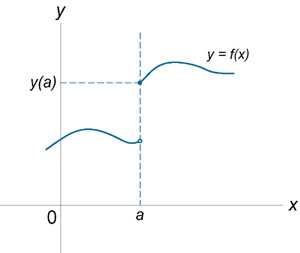
\includegraphics{img/fig1.jpg}
  \caption{Example property graph}
  \label{fig:property-graph}
\end{figure}

For instance, on figure~\ref{fig:property-graph} there are two nodes with labels ``Person'' and ``Company'', respectively. The company has a property ``name'' with a value of ``JetBrains'', and there is an edge from the person to the company labeled ``WORKS\_FOR''. This edge also has a property ``since'' with a value of ``2022''.

% % Рисунок, размещенный с предпочтением "вверху страницы"
% \begin{figure}[t]
% \label{discontinuities}
% \centering
% 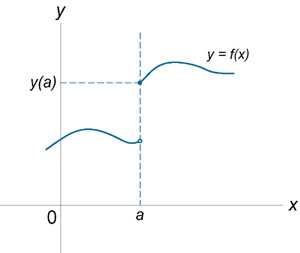
\includegraphics{img/fig1.jpg}
% \caption{Discontinuity}
% \end{figure}

% У заключения нет номера главы
\section*{Conclusion}
\lipsum[1-2]

\setmonofont[Mapping=tex-text]{CMU Typewriter Text}
% \bibliographystyle{plain}
% \bibliography{thesis}
\printbibliography
\end{document}
